\chapter{Experimentación}\label{chapter:experiments}

En este capítulo se presentan tres marcos experimentales con el objetivo de verificar que es posible evaluar sistemas AutoML en los conjuntos de datos de 
\textit{HAutoML-Bench}. 

El primer marco (\ref{section:data}) realiza un análisis visual de las propiedades que presentan dichos conjuntos. El propósito de esta experimentación es mostrar que 
existe complejidad y diversidad en sus propiedades. Esto permite asegurar que se tiene un conjunto de calidad en donde su estrategia de creación mitiga los sesgos de 
selección.

Los dos marcos restantes proponen una evaluación cualitativa y cuantitativa de los sistemas de aprendizaje automático.
La evaluación cualitativa (\ref{section:qualitative}) tiene el fin de efectuar un estudio sobre las características de las herramientas de AutoML. La tarea es determinar 
cuáles herramientas poseen las funcionalidades necesarias para evaluarse en cada uno de los datasets de \textit{HAutoML-Bench}.

El último marco (\ref{section:quantitative}), el de evaluaciones cuantitativas, efectúa las mediciones de rendimiento de los sistemas seleccionados en el marco experimental anterior. En su inicio 
se especifican las diferentes etapas de evaluación y sus configuraciones (\ref{subsection:seetings}). Luego se presentan los valores de 
rendimiento obtenidos y las comparaciones realizadas (\ref{subsection:results}).

En la última sección se discuten los resultados de cada uno de los marcos experimentales (\ref{subsection:discussions}).  

\section{Análisis de los Conjuntos de Datos}\label{section:data}

\textit{HAutoML-Bench} está formado por 11 conjuntos multimodales y 11 conjuntos de texto puro.
La estrategia de selección de estos conjuntos asegura que sus selecciones son un reto para los sistemas AutoML.
Su fortaleza se hace presente en la mezcla de varios dominios y en la presencia de datos no estructurados en sus conjuntos. 
En las figuras (\ref{fig:columns-t},\ref{fig:columns-d},\ref{fig:columns-i},\ref{fig:columns-e}) se muestra que los dataset de evaluación poseen una gran cantidad de 
datos no estructurados y que estas se unen a las característica 
tabulares\footnote{Columnas que son numéricas,booleanas y categóricas} (\ref{fig:columns-n},\ref{fig:columns-b},\ref{fig:columns-c}) para dar más complejidad a la tarea.

Otro de los puntos de dificultad de los dataset de \textit{HAutoML-Bench} son sus metacaracterísticas. Cuando estas propiedades presentan
variedad, aseguran que todo el conjunto está formado por varias muestras representantivas del total de problemas de la vida real.

En la figura \ref{fig:columns} se muestran los diferentes números de columnas que presenta cada dataset siendo \textit{google-guest} el mayor con 40. 
Los números que más predominan son 2 y 3. 
Con respecto a la cantidad de instancias (\ref{fig:instances}) se puede ver que hay conjuntos pequeños, grandes y medianos.
El mayor de todos es \textit{project-kickstarter} y el menor \textit{wnli-es}.
Los valores faltantes (\ref{fig:null}) están presentes en la minoría de los conjuntos; sin embargo, en cada uno de ellos hay una 
gran cantidad de los mismos. 
En los ejemplos de clasificación existe un balance entre los de clasificación binaria y multiclase ((\ref{fig:clases})). De las tareas de clasificación unas de sus 
propiedades más interesantes son el número de conjuntos que poseen desequilibrio (\ref{fig:balance}) y el grado que presentan, es muchos menor que 0.4 porciento. 


\begin{figure}
  \begin{minipage}[b]{0.31\textwidth}
    \centering
    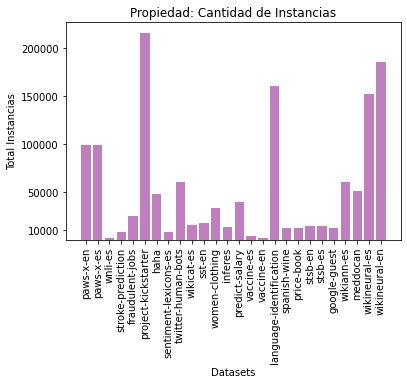
\includegraphics[width=\textwidth]{Graphics/results/instances.png}
      \caption{Instancias}
      \label{fig:instances}
    \end{minipage} 
\hspace{0.01cm}
  \begin{minipage}[b]{0.31\textwidth}
    \centering
      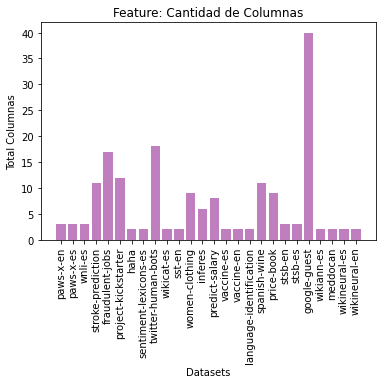
\includegraphics[width=\textwidth]{Graphics/results/columns.png}
        \caption{Columnas}
        \label{fig:columns}
  \end{minipage}      
\hspace{0.01cm}
  \begin{minipage}[b]{0.31\textwidth}
    \centering
      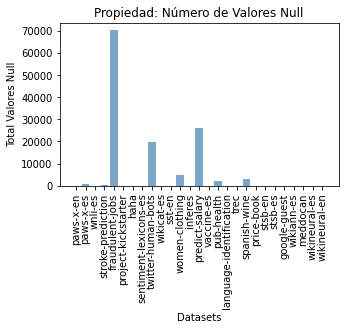
\includegraphics[width=\textwidth]{Graphics/results/null_values.png}
        \caption{Null}
        \label{fig:null}
    \end{minipage} 
\end{figure}

\begin{figure}
  \centering
    \begin{minipage}[b]{0.31\textwidth}
        \centering
        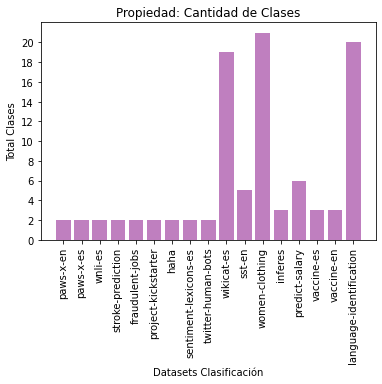
\includegraphics[width=\textwidth]{Graphics/results/class.png}
          \caption{Clases}
          \label{fig:clases}
    \end{minipage}      
\hspace{0.03cm}
    \begin{minipage}[b]{0.31\textwidth}
        \centering
        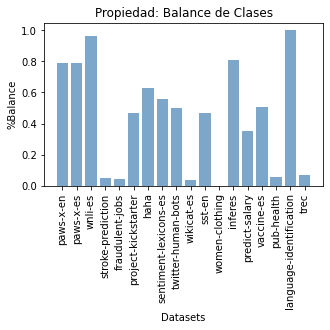
\includegraphics[width=\textwidth]{Graphics/results/balance.png}
          \caption{\% Balance}
          \label{fig:balance}
        \end{minipage} 
      \end{figure}

\begin{figure}
  \centering
    \begin{minipage}[b]{0.31\textwidth}
        \centering
        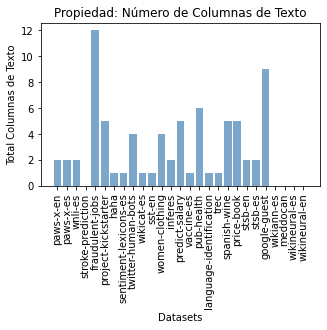
\includegraphics[width=\textwidth]{Graphics/results/columns_t.png}
          \caption{Columnas: Texto}
          \label{fig:columns-t}
    \end{minipage}      
\hspace{0.03cm}
    \begin{minipage}[b]{0.31\textwidth}
        \centering
        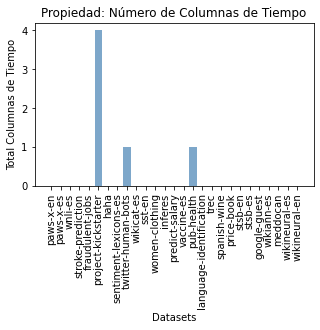
\includegraphics[width=\textwidth]{Graphics/results/columns_d.png}
          \caption{Columnas: Tiempo}
          \label{fig:columns-d}
        \end{minipage} 
\end{figure}

\begin{figure}
  \centering
    \begin{minipage}[b]{0.31\textwidth}
        \centering
        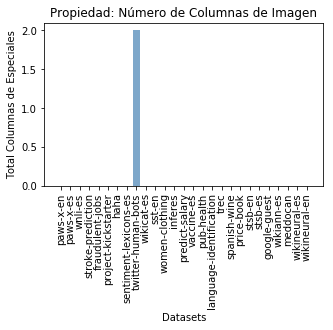
\includegraphics[width=\textwidth]{Graphics/results/columns_i.png}
          \caption{Columnas: Imagen}
          \label{fig:columns-i}
    \end{minipage}      
\hspace{0.03cm}
    \begin{minipage}[b]{0.31\textwidth}
        \centering
        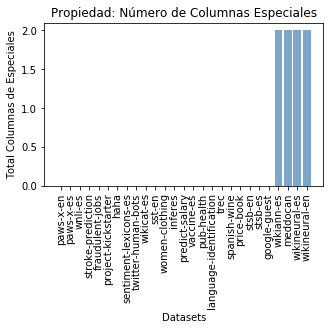
\includegraphics[width=\textwidth]{Graphics/results/columns_e.png}
          \caption{Columnas: Especiales}
          \label{fig:columns-e}
        \end{minipage} 
\end{figure}

\begin{figure}
  \centering
    \begin{minipage}[b]{0.31\textwidth}
        \centering
        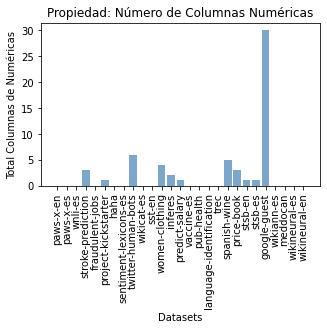
\includegraphics[width=\textwidth]{Graphics/results/columns_n.png}
          \caption{Columnas: Numericas}
          \label{fig:columns-n}
    \end{minipage}    
\hspace{0.01cm}
    \begin{minipage}[b]{0.31\textwidth}
      \centering
      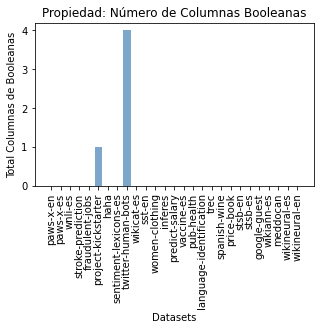
\includegraphics[width=\textwidth]{Graphics/results/columns_b.png}
        \caption{Columnas: Boleanas}
        \label{fig:columns-b}
  \end{minipage}      
\hspace{0.01cm}
    \begin{minipage}[b]{0.31\textwidth}
        \centering
        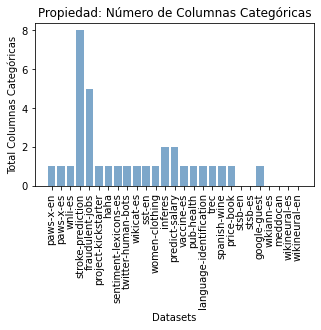
\includegraphics[width=\textwidth]{Graphics/results/columns_c.png}
          \caption{Columnas: Categoricas}
          \label{fig:columns-c}
        \end{minipage} 
\end{figure}

\section{Evaluaciones Cualitativas}\label{section:qualitative}

En los últimos años se han desarrollado una gran cantidad de marcos de aprendizaje automático, ya sea mediante la mejora iterativa de diseños antiguos o mediante 
el uso de enfoques novedosos. Estos se clasifican atendiendo a sus características internas y externas [\cite{52}]. Las características internas definen su 
funcionamiento, tales como el tipo y la variedad de algoritmos sobre los cuales realizan la búsqueda. Las externas 
destacan la utilidad de los sistemas. En esta categoría se encuentran los dominios a los que son aplicables. También las tareas que resuelven, ya sean las clásicas de 
aprendizaje automático o las específicas de dominios: relacionadas con imágenes, textos y series temporales. 

La unión de las características internas y externas determinan cuan eficientes y rápidos son los sistemas, aún más importante determinan qué problemas de la 
vida real resuelven.
Los problemas que agrupa \textit{HAutoML-Bench} poseen una complejidad en su estructura debido a la naturaleza de sus datos. Además, 
requieren técnicas de sus dominios de aplicación para su resolución. Este benchmark va dirigido a sistemas AutoML que sean capaces de flexibilizar sus tipos de entrada 
y que contengan los algoritmos necesarios para atacar la mayor cantidad de tareas. 

Se propone realizar un estudio de herramientas de AutoML para identificar cuáles pueden evaluarse en \textit{HAutoML-Bench} solo atendiendo a sus características.
Aunque existe una gran cantidad de herramientas de AutoML, solo se analiza una selección entre todas las existentes.

%Auto-Weka
Auto-Weka[\cite{8}] es uno de los primeros sistemas en darse a conocer, utiliza la biblioteca de aprendizaje Weka y está implementado en el lenguaje Java. 
Su estrategia de recorrido del Espacio de Búsqueda está encaminado a los algoritmos basados en optimización bayesiana. El mismo está formado por modelos de ML 
clásicos, ya sean lineales, basados en árboles, ensambles y otras familias. Sus técnicas de preprocesamiento son deficientes y con respecto al dominio son nulas, 
lo limitan a enfrentarse solo a problemas tabulares.

%AutoSklear
Auto-Sklearn[\cite{9}] extiende la propuesta de Auto-Weka en mejoramientos de eficiencia y Robustez. Ambos incluyen como estrategia de búsqueda la optimización 
bayesiana. Una de sus diferencias radica en la biblioteca de algoritmos, ya que este se implementa sobre Scikit-Learn de Python. Además incluye meta-aprendizaje. 
Las técnicas de preprocesamiento de Auto-Sklearn son superiores a las de Auto-Weka, aun así solo puede ser aplicable a problemas en donde sus datos tienen forma 
numérica y/o categórica. 

%TPO y RECIPE
El marco TPOT [\cite{65}] comparte las limitaciones mencionadas y al igual que Auto-Sklearn está implementado sobre Scikit-Learn, pero también incluye un algoritmo de 
la biblioteca XGBoost. Su mayor diferencia con los anteriores es su estrategia de Búsqueda, la cual se basa en programación evolutiva. 
El sistema RECIPE [\cite{64}] comparte las características anteriores con TPOT incluyendo sus limitaciones. Este también se encuentra restringido a problemas que se 
modelan con datos estructurados y con propiedades tabulares. Sin embargo, posee una desventaja respecto a los anteriores y es que solo es aplicable a problemas de 
clasificación, mientras que Auto-Weka, Auto-Sklearn y TPOT permiten adicionalmente regresión. Entre las ventajas de RECIPE se encuentra que al utilizar una 
gramática para organizar el conocimiento adquirido sobre las exitosas canalizaciones creadas, evita la generación de canalizaciones no válidas. Además de que el 
espacio de búsqueda es mayor con respecto a los anteriores.

Se puede observar que estos 4 sistemas como características comunes presentan que los datos de entrada deben contener solo características tabulares.
Los conjuntos del benchmark no evalúan esta cualidad de manera independiente de los demás dominios. Además, incluyen una variedad de tipos de tareas como 
reconocimiento de entidades, procesamiento del lenguaje natural que van más allá de una simple clasificación o regresión. Las tareas que modelan 
exigen técnicas del dominio al que pertenecen. Estas propiedades afirman que Auto-Weka, Auto-Sklearn, TPOT y RECIPE carecen de flexibilidad para 
su evaluación en todos los conjuntos de \textit{HAutoML-Bench}.

Los sistemas que solo utilizan redes neuronales para su modelado también son sistemas AutoML. Los más utilizados son Auto-Keras[\cite{13}] y Auto-Pytorch[\cite{21}], 
ambos se basan en la optimización bayesiana. 
AutoPytorch[\cite{21}] como su nombre lo indica, está implementado sobre el framework Pytorch. Este incluye redes neuronales y técnicas de ensamble. 
Las técnicas de preparación de características y del dominio que posee lo resalta del resto en su categoría de sistema AutoDL. Además de que puede ser aplicado a 
problemas de clasificación y regresión sin muchas modificaciones.

Auto-Keras[\cite{13}] se encuentra implementado sobre la biblioteca Keras. Este, al igual que AutoPytorch en sus respectivas evaluaciones de lanzamiento, 
se evaluaron en conjuntos de dominio imagen y tabular. A pesar de esto, en el bechmark no existen conjuntos que solamente respondan a esos tipos. 
Auto-Keras tiene componentes para tratar con el dominio texto y problemas multimodales, sobre AutoPytorch no hay indicios de que sea flexible 
ante estos. 
Auto-Keras dice poder enfrentarse a conjuntos de texto y multimodales y en sus ejemplos de uso solo se demuestra con conjuntos juguetes, los cuales carecen de 
semántica al estar transformados. En conclusión, no existe evidencia de que el sistema pueda evaluarse en datasets en donde los datos se encuentran no estructurados. 

Por último, dos sistemas que son relativamente nuevos y que incluyen ambos enfoques: modelos de machine learning clásico y redes neuronales. 
Estos sistemas son AutoGOAL y AutoGluon.

AutoGOAL[\cite{40},\cite{41}] es una propuesta de AutoML heterogéneo que construye un espacio de búsqueda jerárquico mediante gramáticas libres del contexto y 
probabilidades. A diferencia de los anteriores sistemas, posee un proceso de introspección de código que se encarga de explorar sus bibliotecas base en búsqueda de 
algoritmos, en vez de utilizar implementaciones directas de las mismas. Sus bibliotecas base son Scikit-learn, Nltk, Keras, Gensim y Pytorch. Resuelve tareas clásicas 
de machine learning como clasificación, regresión y clustering. Además, problemas relacionados con dominios específicos como procesamiento del lenguaje natural. También 
resuelve tareas con imágenes y tabulares puros, como un extra permite resolver problemas de reconocimiento de entidades y relaciones.Su implementación de tipos 
semánticos para la declaración de la entrada y salida de los problemas le permite utilizar datos estructurados y no estructurados. Sus tipos y la forma en que construye 
y recorre el espacio de búsqueda es lo que le permite resolver el problema de AutoML Heterogéneo. Existe evidencia de que AutoGOAL puede evaluarse en tareas de  NLP, 
en conjuntos de datos que contienen una y más columnas de texto. Sin embargo, en conjuntos de datos multimodales carecen de un tipo definido que permita modelar estas 
entradas.   

AutoGluon[\cite{17},\cite{42}] es un sistema AutoML el cual definen de antemano los posibles modelos y las formas de combinarlos para construir su espacio de búsqueda.
Se adapta a varios modelos que van desde árboles potenciados listos para usar hasta modelos personalizados de redes neuronales [\cite{37}]. Tiene modelos predictores 
para tipo de datos imágenes, texto, datos tabulares y series temporales. AutoGluon es capaz de predecir cual de los modelos usar en dependencia de la entrada.
Este posee una inferncia de tipos bastante robusta. Es capaz de inferir los tipos de las columnas de entrada de texto, series temporales, numéricas, categóricas y 
booleanas. Además, a partir de la columna salida infiere el tipo de tarea. AutoGluon puede resolver problemas de ML clásicos y también específicos de un dominio. En 
sus evaluaciones se recogen problemas tabulares, de procesamiento del lenguaje natural y de imágenes. Recientemente con su modelo Multimodal es capaz de resolver 
problemas multimodales en donde los tipos de datos de imágenes, texto y tabulares se encuentran en gran escala. Desde antes con su modelo Tabular, estos tipos de 
problema podían resolverse para columnas de texto y tabulares, estas últimas deben representar la mayoría. 
Se puede decir que por sus características AutoGluon está preparado para enfrentarse a los conjuntos multimodales y de texto de \textit{HAutoML-Bench} excepto a las 
tareas de reconocimiento de entidades. AutoGluon tiene técnicas para tratar las tareas de econocimiento de entidades; sin embargo, la entrada para este tipo de problemas
presentan una estructura diferentes a las que poseen los conjuntos de \textit{HAutoML-Bench}.  

En la figura \ref{fig:eval-cuali} se muestran un resumen de las tareas en donde las propiedades de los sistemas permiten resolver. 
\begin{table}[H]
  \centering
  \resizebox{10cm}{!} {
  \begin{tabular}{|l|c|c|c|c|c|}
  \hline
  Dataset & \multicolumn{3}{c|}{Texto} & \multicolumn{2}{c|}{Multimodales}\\ \hline
                        & Clasif   & Regres   & Entidades& Clasif   & Regres   \\ \hline
  Auto-Weka             &          &          &          &          &          \\
  Auto-Sklearn          &          &          &          &          &          \\
  TPOT                  &          &          &          &          &          \\ 
  RECIPE                &          &          &          &          &          \\
  AutoPytorch           &          &          &          &          &          \\
  Auto-Keras            &          &          &          &          &          \\
  AutoGOAL              &\checkmark&\checkmark&\checkmark&          &          \\
  AutoGluon             &\checkmark&\checkmark&          &\checkmark&\checkmark\\ \hline
  &  10      &  2       &  4       &   8      &  3       \\ \hline
  \end{tabular}
  \caption{Evaluación Cualitativa de los sistemas sobre los conjuntos de datos del benchmark}
  \label{fig:eval-cuali}
  }
\end{table}

\section{Evaluaciones Cuantitativas}\label{section:quantitative}

Las evidencias presentadas en el apartado (\ref{section:qualitative}) permiten concluir que AutoGOAL y AutoGluon atendiendo a sus características pueden 
evaluarse en 16 y 23 conjuntos de \textit{HAutoML-Bench} respectivamente.
Para la evaluación cuantitativa, el sistema seleccionado es AutoGluon. Este posee inicialmente la mayor cantidad de tareas que sus características afirman puede resolver. 
La selección incluye solo uno de los sistemas debido a limitantes de tiempo y software. 
En las próximas subsecciones se explica todo el marco experimental cuantitativo que pone a prueba el rendimiento de AutoGluon (\ref{subsection:seetings}). Se muestran 
los resultados del rendimiento del sistema (\ref{subsection:results}) y se explican los errores que surgieron en las evaluaciones (\ref{subsection:errors})

\subsection{Descripción y Configuración de las Evaluaciones}\label{subsection:seetings}

La experimentación cuantitativa propone realizar tres rondas de evaluaciones de AutoGluon sobre todos los conjuntos de datos.

La primera ronda tiene como objetivo medir el rendimiento de AutoGluon con todos sus parámetros de entrada en sus valores por defecto. En esta solo se especifican los 
relacionados con la métrica de optimización y el tiempo de entrenamiento. 

La segunda ronda pretende evaluar el sistema en las mismas condiciones de la primer ronda, excepto por el tiempo que pretende superar el anterior.
Estas primeras etapas de ejecuciones tienen como fin evaluar al sistema realizando su propia inferencia de tipos, se pretende que la herramienta obtenga la mínima
ayuda externa. La segunda, su objetivo más importante es verificar si el rendimiento de la herramienta es sensible a los cambios de tiempo, posibilitando alguna 
mejora en la mayoría de los conjuntos.

En la última ronda se introducen como entrada los tipos semántico de cada columna de los dataset. La meta es validar la consistencia de los resultados de AutoGluon en 
comparación con los obtenidos con inferencia de tipos durante el mismo tiempo de entrenamiento. 

En la subsección \ref{seetings:hadware} se presenta el entorno de ejecución en donde se realizan las pruebas y en la subsección \ref{seetings:marcos} se definen las 
configuraciones adicionales del sistema. 

\begin{flushleft} 
  { \textbf{Hadware}}\label{seetings:hadware}
\end{flushleft}

El hadware de evaluación seleccionado es la plataforma Colab. Esta cuenta con un entorno de ejecución en la nube que provee recursos para ejecutar programas 
escritos en el lenguaje Python. Los recursos presentes en la evaluación son: CPU de 12 GB de RAM máximo, 120 GB de almacenamiento de disco duro y 188 unidades de GPU.


\begin{flushleft} 
  { \textbf{Configuración del Sistema AutoML}}\label{seetings:marcos}
\end{flushleft}

AutoGluon se utiliza en su versión estable v0.5.2. Esta herramienta tiene muchos parámetros configurables en cada uno de sus modelos, tabular, multimodal, imagen y texto. 
Estos presentan su configuración predeterminada, exceptuando los que se describen a continuación.
\begin{itemize}
    \item Restricciones de software: AutoGluon se instala con GPU en vista a verificar su rápidez y rendimiento durante las pruebas. No existen limitaciones de RAM salvo
    las inpuestas por el entorno de ejecución.
    \item Métrica de optimización: Se utilizan para clasificación binaria: F1, clasificación multiclase: accuracy y para regresión el error cudrático medio. Todas se 
    ecuentran dentro de las métricas medidas en la evaluación. Se emplean estas y no las ideales recomendadas porque AutoGluon es restrictivo con las métricas que 
    pueden utilizarse en cada modelo. La \textit{balanced-accuracy} está fuera de las permitidas.
    \item Restricciones de tiempo: selección de dos instantes de tiempo para la realización de las evaluaciones 5 min y 15 min. 
    \item Tamaño del conjunto de validación: utilizar un tamaño 0.2 del total de instancias que equivale a un 20\%. 
    \item Parámetros obligatorios: la etiqueta de la columna salida.  
\end{itemize}


\subsection{Resultados}\label{subsection:results}
AutoGluon realiza 3 etapas de evaluaciones sobre los conjuntos de datos. La primera y la segunda con sus parámetros por defecto y un tiempo de 5 y 15 minutos de entrenamiento
por conjunto respectivamente. La tercera se realiza durante 5 minutos por conjunto introduciendo como entrada el tipo de las columnas. 

Los valores obtenidos durante cada una de estas etapas se muestran en esta sección. Los resultados se encuentran separados en los diferentes tipos de tareas
en las figuras (\ref{fig:class-binary}, \ref{fig:class-multi}, \ref{fig:regression}) que corresponden a clasificación binaria, multiclase y regresión.  

Las métricas de evaluación que se muestran para cada tarea es la utilizada para la optimización del sistema y la métrica ideal propuesta en la 
sección(\ref{subsection:metrics}). Recordar que para las tareas de clasificación es \textit{balanced-accuracy} y para regresión \textit{RMSE}.
En el caso de la regresión, los valores de la variable de salida no se encuentran en el mismo rango, ni los resultados obtenidos en la métrica \textit{RMSE} 
durante la evaluación del benchmark. Producto a esto, los valores del error de un conjunto impiden su comparación. Para resolver este inconveniente,
como evaluación independiente\footnote{Los resultados originales junto a las otras métricas que se excluyeron en esta descripción se encuentran en el repositorio del 
benchmark.} se estandarizan los valores de las variables de salida y las predicciones de cada conjunto de regresión, luego se calcula la métrica 
\textit{RMSE}.

En las figuras tambíen se muestra el promedio de los resultados de cada métrica en cada tarea. Este promedio permite analizar de manera general los cambios que 
sufren los valores de rendimiento de AutoGluon en las 3 etapas de evaluaciones.

En esta sección se ofrece una descripción de los resultados obtenidos en todas las etapas de la evaluación en cada uno de los tipos de tareas por 
separado (\ref{results:task}). 
Luego se compara el rendimiento del sistema en las distintas etapas (\ref{results:comparation}). Las comparaciones se efectuan ente aquellas que 
mantienen sus parámetros por defecto y existe un aumento del tiempo (etapa 1 y 2). 
También cuando se mantiene el mismo tiempo y lo que varía es la introducción de los tipos de las columnas de entrada (etapa 1 y 3).


\begin{flushleft} 
  {\large { \textbf{Resultados de AutoGluon por Tipo de Tarea}}}\label{results:task}
\end{flushleft}

Los resultados en las distintas tareas se manifiestan similares en cada una de las etapas. Esta similitud es teniendo en cuenta los mejores y peores conjuntos en 
rendimiento.

En la clasificación atendiendo a los valores de la métrica \textit{balanced-accuracy} común en ambas, el mayor promedio de desempeño durante tdas rondas de evaluación 
lo posee la clasificación binaria.

En esta tarea, el conjunto en el que AutoGluon tiene mejor rendimiento durante todos las evaluaciones es \textit{paw-x-en}. Los peores resultados varían en dependencia de la etapa y la 
métrica. El que más resalta es \textit{stroke-prediction} que posee un valor de \textit{F1} igual a cero durante todas las etapas. Las evaluaciones del conjunto 
\textit{fradulent-job} tienen un comportamiento similar excepto en la etapa 2 en donde aumenta el valor de su rendimiento. En la métrica \textit{balanced-accuracy} 
los conjuntos \textit{project-kickstarter} y \textit{wnli-es} se unen a aquellos en donde el rendimiento es malo.

En la clasificación multiclase, al igual que en la clasificación binaria, existe un conjunto en donde AutoGluon tiene buenos resultados durante todas las rondas de 
ejecuciones. Este es \textit{language-identification}. En la tercera ronda de evaluaciones el mejor rendimiento es compartido con \textit{trec}. El peor desempeño 
durante todo el proceso es en el conjunto \textit{predict-salary}.

En la tarea regresión los mejores resultados los obtiene AutoGluon en el conjunto \textit{stsb-en}, mientras que el error es mayor en \textit{price-book} de manera 
general para todas las rondas de ejecuciones.


\begin{flushleft} 
  {\large { \textbf{Comparación de los Resultados de las Etapas de Evaluación de AutoGluon}}}\label{results:comparation}
\end{flushleft}


La evaluación de los conjuntos de una etapa a la otra poseen poca variabilidad.  

Los resultados del sistema con sus parámetros de entrada por defecto, muestran un promedio de desempeño superior en 15 minutos que en 5 minutos. 
En todos los conjuntos de clasificación binaria, AutoGluon aumenta su rendimiento con el incremento del tiempo. 
Las variaciones mayores en este tipo de tareas son en los conjuntos \textit{fradulent-job} y \textit{project-kickstarter}, mientras que \textit{stroke-prediction}, 
es el único en donde no se observa una variación en sus resultados.

En la clasificación multiclase existe una disminución del rendimiento del sistema, a medida que aumenta el tiempo, en los conjuntos \textit{predict-salary} y 
\textit{vaccine-es}. En todos los conjuntos restantes de esta categoría, sus valores de eficiencia muestran un aumento, el mayor de todos es en el 
conjunto \textit{wikicat-es}.

En las dos tareas de clasificación, el cambio en los valores de eficiencia de un tiempo a otro es más significativo en la clasificación binaria.

En estas etapas, las tareas de regresión  mejoran sus resultados en todos sus conjuntos, excepto \textit{price-book}.

AutoGluon con La introducción de los tipos de datos de las columnas de los conjuntos en la etapa 3, no muestra una gran variación en sus resultados.
Este en la mayoría de los dataset tiende a mantener o disminuir su eficiencia al tener como entrada los tipos de las columnas. Los conjuntos en los que muestra un 
notable incremento en su rendimiento son \textit{project-kickstarter} en clasificación binaria, en multiclase \textit{women-clothing} y regresión 
\textit{google-guest}. Estos grandes incrementos provocan que el promedio de rendimiento de la tercera etapa sea mayor al de la primera. Si bien el promedio es mayor, 
esto no significa, que para los conjuntos sea favorable el introducir como entrada el tipo de las columnas. 
AutoGluon en la tarea regresión muestra su mayor disminución de eficiencia de una etapa a la otra en el conjunto \textit{spanish-wine}.

\begin{table}
  \centering
  \resizebox{15cm}{!} {
  \begin{tabular}{|l|cccccc|}
  \hline
          & \multicolumn{4}{p{8cm}|}{Tiempo: 5 min}  & \multicolumn{2}{p{4cm}|}{Tiempo: 15 min}\\  \hline
          & \multicolumn{2}{p{4cm}|}{Valores por defecto} & \multicolumn{2}{p{4cm}|}{Entradad de Tipo} & \multicolumn{2}{p{4cm}|}{Valores por defecto}\\ \hline
  Dataset & F1 & bala-acc & F1  & bal-acc & F1 & bal-acc  \\ \hline
  paws-x-en             & 0.931 & 0.940 & 0.917 & 0.928 & 0.947 & 0.953 \\
  paws-x-es             & 0.840 & 0.856 & 0.837 & 0.852 & 0.875 & 0.888 \\
  wnli-es               & 0.61  & 0.5   & 0.613 & 0.5   & 0.613 & 0.5   \\ 
  stroke-prediction     & 0.0   & 0.5   & 0.0   & 0.5   & 0.0   & 0.5 \\
  fraudulent-jobs       & 0.0   & 0.5   & 0.0   & 0.5   & 0.732 & 0.818 \\
  project-kickstarter   & 0.074 & 0.498 & 0.225 & 0.499 & 0.153 & 0.502 \\
  haha                  & 0.764 & 0.807 & 0.761 & 0.803 & 0.774 & 0.814 \\
  sentiment-lexicons-es & 0.747 & 0.770 & 0.747 & 0.770 & 0.775 & 0.794 \\ 
  twitter-human-bots    & 0.680 & 0.770 & 0.676 & 0.759 & 0.721 & 0.791 \\ \hline
  \textbf{Promedio}     & 0.516 & 0.682 & 0.530 & 0.679 & 0.621 & 0.728 \\ \hline


  \end{tabular}
  \caption{Resultados en tareas de Clasificación Binaria}
  \label{fig:class-binary}
  }
\end{table}

\begin{table}
  \centering
  \resizebox{15cm}{!} {
    \begin{tabular}{|l|cccccc|}
  \hline
          & \multicolumn{4}{p{8cm}|}{Tiempo: 5 min}  & \multicolumn{2}{p{4cm}|}{Tiempo: 15 min}\\  \hline
          & \multicolumn{2}{p{4cm}|}{Entrada: Defecto} & \multicolumn{2}{p{4cm}|}{Entrada: Tipos} & \multicolumn{2}{p{4cm}|}{Entrada: Defecto}\\ \hline
          Dataset & acc & bala-acc & acc  & bal-acc & acc & bal-acc  \\ \hline
  wikicat-es              & 0.385 & 0.268 & 0.385 & 0.268 & 0.603 & 0.518 \\
  sst-en                  & 0.580 & 0.549 & 0.580 & 0.549 & 0.577 & 0.545 \\
  women-clothing          & 0.671 & 0.449 & 0.677 & 0.456 & 0.760 & 0.642 \\ 
  inferes                 & 0.691 & 0.680 & 0.651 & 0.647 & 0.767 & 0.759 \\
  predict-salary          & 0.199 & 0.178 & 0.190 & 0.173 & 0.191 & 0.172 \\
  language-identification & 0.966 & 0.966 & 0.966 & 0.966 & 0.976 & 0.976 \\
  vaccine-es              & 0.780 & 0.756 & 0.779 & 0.743 & 0.779 & 0.766 \\
  pub-health              & 0.609 & 0.370 & 0.609 & 0.370 & 0.759 & 0.576 \\ 
  trec                    & 0.962 & 0.912 & 0.966 & 0.933 & 0.970 & 0.972 \\ \hline
  \textbf{Promedio}       & 0.649 & 0.569 & 0.723 & 0.567 & 0.684 & 0.658 \\ \hline


    \end{tabular}
  \caption{Resultados en tareas de Clasificación Multiclase}
  \label{fig:class-multi}
  }
\end{table}

\begin{table}
  \centering
  \resizebox{15cm}{!} {
  \begin{tabular}{|l|ccc|}
  \hline
  & \multicolumn{2}{p{8cm}|}{Tiempo: 5 min}  & \multicolumn{1}{p{4cm}|}{Tiempo: 15 min}\\  \hline
  & \multicolumn{1}{p{4cm}|}{Entrada: Defecto} & \multicolumn{1}{p{4cm}|}{Entrada: Tipos} & \multicolumn{1}{p{4cm}|}{Entrada: Defecto}\\ \hline
               & RMSE  & RMSE  & RMSE  \\ \hline
  spanish-wine & 0.8274  & 36.62  & 0.5581 \\
  stsb-en      & 0.4548  & 0.472  & 0.4349 \\
  stsb-es      & 0.6265  & 0.6265 & 0.6231   \\ 
  price-book   & 32.537  & 40.675 & 40.864  \\
  google-guest & 1.7156  & 1.5171 & 1.5355  \\ \hline
  \textbf{Promedio} & 0.1741 & 0.1652 & 0.1556 \\ \hline

\end{tabular}
  \caption{Regresión}
  \label{fig:regression}
  }
\end{table}


\subsection{Errores de los sistemas durante el marco experimental}\label{subsection:errors}
AutoGluon presenta fallas durante las ejecuciones de algunos conjuntos. Estos para poder evaluarse tienen que ser sometidos a transformaciones.

El dataset \textit{women-clothing} contiene una clase que solo posee una intancia. También posee valores faltantes en su columna salida. En ambos casos AutoGluon se 
limita a resolver problemas de este tipo. Para que el sistema pueda ejecutarse las instancias con problemas son removidas.

El conjunto \textit{google-guest} tiene en su etiqueta final un número de valores distintos bastante pequeño. En su definición original este modela una tarea de regresión, en 
donde los valores de la etiqueta final pueden estar en el rango [0,1]. AutoGluon infiere incorrectamente el tipo de tarea, lo que produce errores en la ejecución, para 
dar una solución se introduce el tipo de tarea solamente para este conjunto.

Estas ejecuciones fallidas ocurren durante la primera ronda de pruebas. Las soluciones a estos problemas deben ser utilizadas en las restantes rondas. 
En la última ocurren errores al introducir los tipos semánticos de cada una de las columnas. Las primeras limitaciones se dan al no poder introducir como 
parámetro de entrada el tipo \textit{datetime}, que hace referencia a los tipos de tiempo y fecha. Además, en el procesamiento del tipo \textit{path\_image} de AutoGluon. 
Este solo permite imágenes ubicadas en un directorio, carece de la funcionalidad de descargar imágenes de una url.  Esrtos tipos fueron apartados de la entrada.

El conjunto \textit{spanish-wine} en sus entradas etiquetadas como numéricas y que presentan datos faltantes AutoGluon detiene la ejecución. Al ser pocas instancias 
se remueven.
En el caso de \textit{price-book} contiene columnas que su tipo semántico es numeral y su tipo concreto es cadena de texto. AutoGluon carece de técnicas para 
enfrentarse a este tipo de situaciones. En este ejemplo se transformaron las columnas a números y se le pasaron al sistema de esa forma.

En todas las rondas de evaluaciones existieron errores de falta de RAM, la plataforma Colab se reinicia constantemente producto al gasto excesivo de recursos. Los 
experimentos no pudieron ejecutarse secuencialmente debido a esta limitante.

\section{Discusiones}\label{subsection:discussions}

Las evaluaciones cuantitativas y cualitativas realizadas en las secciones (\ref{section:quantitative}) y (\ref{section:qualitative}) denotan la complejidad que poseen 
los conjuntos de \textit{HAutoML-Bench}.
El análisis que se realiza sobre sus propiedades ya habían anticipado su dificultad, producto a los tipos de datos no estructurados que poseen y a sus metacaracterísticas.

Las experimentaciones cualitativas evidencian que en su mayoría los sistemas AutoML son incapaces de evaluar su eficiencia en los conjuntos de \textit{HAutoML-Bench}. 
En los casos de la herramienta AutoDL, que ya poseen técnicas para procesar tareas de un dominio específico, deben agregar técnicas para lidiar con datos no estructurados. 
En los ejemplos de sistemas AutoML que solo se ejecutan en datos tabulares, deben desprenderse de esta limitante con el fin de lograr la heterogeneidad. 
El sistema AutoGOAL debe añadir más tipos semánticos para poder evaluarse en dataset multimodales. AutoGluon debe ampliar las formas en que recibe el tipo de entrada 
de las tareas de reconocimiento de entidades.

AutoGluon es el sistema con características más maduras que permiten la evaluación en 23 conjuntos de datos de \textit{HAutoML-Bench}.
Los resultados de su evaluación cuantitativa presenta algunas de las deficiencias que este sistema aún posee. Además, resalta sus fortalezas, ya que obtuvo buenos resultados 
en algunos casos.

Los valores de rendimiento que obtiene el sistema, buenos o malos, se agrupan, atendiendo a las características que presentan los datos en cada conjunto.

Los buenos resultados de AutoGluon suelen ser en conjuntos con un índice de balance elevado en sus clases. Ejemplo son \textit{paws-x-en} y 
\textit{language-identification} que son los más balaceados de \textit{HAutoML-Bench}. El idioma inglés parece ser otra ventaja para el buen rendimiento.
Existen conjuntos creados para el idioma español y el inglés. Autogluon en todos los casos, obtiene una mayor eficiencia en los de idioma inglés.

El desbalance de clase y los conjuntos multimodales parecen ser la mayor fuente de ineficiencia. Ejemplo son los conjuntos \textit{stroke-prediction} y 
\textit{fraudulent-job}, que durante durante casi todas las etapas de evaluación mantienen un rendimiento bastante bajo e invariante. Ambos solo predicen 
correctamente la clase negativa. El dataset \textit{fraudulent-job} en un intervalo mayor de tiempo que el inicial logra aumentar sus resultados, a pesar de ser un 
conjunto con muchos valores faltantes. AutoGluon parece enfrentar bien estos faltantes cuando la característica no se especifican como numérica. Otra desventaja es los 
pocos datos de entrenamiento en conjuntos multimodales. Los datasets \textit{Wnli-es} y \textit{stroke-prediction} son muestra de esta deficiencia. \textit{Wnli-es} al 
contrario de los anteriores conjuntos mencionados, tiende a predecir con mayor frecuencia la clase positiva.

El rango de los valores de la variable de salida elevado, muestra un aumento en el error del rendimiento de AutoGluon en tareas de regresión. 
Este es el caso de \textit{price-book}. También infieren sus características multimodales. En las tareas de clasificación multiclase, se repiten los bajos rendimientos
en tareas multimodales, con valores faltantes y desbalance de clase. Ejemplo el conjunto \textit{predict-salary} que obtiene los resultados más bajos de esta tarea. 

Los resultados en todas los conjuntos demuestran la superioridad del rendimiento en tareas de texto puro sobre las multimodales. 

Con respecto a los objetivos de cada etapa de evaluación. En aquellas donde se comparan los resultados con diferente tiempo, AutoGluon demuestra un aumento en 
su rendimiento. Se estima que el tiempo máximo de entrenamiento es suficiente para completar las tareas, considerando que todos los conjuntos se evaluan con GPU y que 
logran alcanzar como mínimo la etapa 2 de entrenamiento. En este tiempo, los resultados por tarea, presentan un promedio menor al 75 por ciento. El valor promedio, 
comparado con las épocas de entrenamiento, es ineficiente. 

En las comparaciones en donde se quiere verificar la fortaleza de la inferencia de tipos, AutoGluon demuestra que no existen variaciones drásticas entre las etapas 
comparadas. Existen conjuntos en donde el sistema disminuye su rendimiento cuando se introducen los tipos de entrada. Esto afirma que los tipos que se infieren, 
en muchos casos, no coincide con el correcto, a pesar de ello, AutoGluon se las ingenia para obtener un resultado medio.



% Los buenos resultados de AutoGluon en los conjuntos \textit{paws-x-en} y \textit{language-identification}, son producto a 
% que poseen un elevado índice de balance de clases. El dataset \textit{language-identification} que pertenece a clasificación multiclase se encuentra 
% completamente balanceado, mientras que \textit{paws-x-en} de clasificación binaria posee un índice cercano a 1, el ideal. También, ambos tienen un gran número de 
% instancias, que con un correcto tiempo de entrenamiento significan más información de la que aprender. 

% El conjunto \textit{trec}, en la ejecución de mayor tiempo, se suma a la lista de los mejores resultados. Este, a pesar de poseer un gran desbalance de clases, carece 
% de valores faltantes y no mezcla diferentes tipos de datos. Además, pertenece al idioma inglés, lo que puede influir en sus buenos resultados. AutoGluon tiende a tener 
% mejores resultados en los conjuntos de idioma inglés. Los conjuntos \textit{paws-x-en}, \textit{paws-x-es} de clasificación binaria y los conjuntos \textit{stsb-en} y 
% \textit{stsb-es} de regresión, tratan sobre el mismo ambiente y se encuentran en idioma inglés y español. Ambos afirman la hipótesis de que AutoGluon resuelve con 
% mejor rendimiento, aquellos conjuntos que están en el idioma inglés. El conjunto \textit{stsb-en} es el de mejor rendimiento en la tarea de regresión.

% En el lado opuesto de los dataset mencionados, se encuentran aquellos con malos valores de rendimiento. Entre estos está el dataset \textit{stroke-prediction} que 
% durante ninguna de sus ejecuciones, a lo largo de las distintas etapas, logra aumentar su desempeño. Esto es producto, a que la clase positiva de esta tarea de 
% clasificación binaria posee muy pocos ejemplos de entrenamiento, en comparación con la clase negativa. En este caso, la clase negativa abarca todos los resultados 
% predictivos. El aumento de tiempo para este dataset no significa un avance, ya que el conjunto es pequeño. El dataset logra avanzar hasta la época 5 de evaluación sin 
% cambios en sus resultados. El conjunto \textit{fraudulent-job} se comporta similar a \textit{stroke-prediction} durante las dos primeras etapas. Este en un intervalo 
% mayor de tiempo logra aumentar su rendimiento drásticamente. La diferencia entre ambos conjuntos es que \textit{fraudulent-job} posee un mayor balance y número de 
% instancias, su multimodalidad carece de columnas numéricas. Estas características superan a su gran número de valores faltantes. El dataset \textit{wnli-es} le debe 
% su mal rendimiento a que es el más pequeño de todos los conjuntos. \textit{Wnli-es} al contrario de los anteriores conjuntos mencionados, tiende a predecir con mayor 
% frecuencia la clase positiva.

% En la clasificación multiclase en donde los rendimientos son similares entre todos los conjuntos, \textit{predict-salary} muestra el peor de todos. Este posee 
% valores faltantes y varias columnas categóricas y de texto. En la regresión, el peor es \textit{price-book}, su complejidad está en la mezcla de varios tipos de datos y 
% en el rango en que varían los valores de su variable de salida.

% Los buenos resultados están encabezados por los dataset de texto puro, mientras que los malos en su mayoría son multimodales. La característica que más 
% resulta ser desafiante para AutoGluon, es el desbalance de clases.

% En la mayoría de los conjuntos durante la etapa en que se introducen los tipos de entrada, existe una disminución o mantenimiento de su rendimiento respecto a la etapa
% con parámetros por defecto. Esto, demuestra la fortaleza de la inferencia de tipos de AutoGluon, al no existir variaciones drásticas. 
% Sin embargo, también afirma,